
%(BEGIN_QUESTION)
% Copyright 2015, Tony R. Kuphaldt, released under the Creative Commons Attribution License (v 1.0)
% This means you may do almost anything with this work of mine, so long as you give me proper credit

\noindent
{\bf Lab Exercise -- introduction}

\vskip 5pt

Your task is to add cascade, ratio, or feedforward action to your working process control system.  This will require the addition of another process transmitter as well as additional programming inside the controller.

The following table of objectives show what you and your team must complete within the scheduled time for this lab exercise.  Note how some of these objectives are individual, while others are for the team as a whole:

\underbar{Objective completion table:}

% No blank lines allowed between lines of an \halign structure!
% I use comments (%) instead, so that TeX doesn't choke.

$$\vbox{\offinterlineskip
\halign{\strut
\vrule \quad\hfil # \ \hfil & 
\vrule \quad\hfil # \ \hfil & 
\vrule \quad\hfil # \ \hfil & 
\vrule \quad\hfil # \ \hfil & 
\vrule \quad\hfil # \ \hfil & 
\vrule \quad\hfil # \ \hfil & 
\vrule \quad\hfil # \ \hfil \vrule \cr
\noalign{\hrule}
%
% First row
{\bf Performance objective} & {\bf Grading} & {\bf 1} & {\bf 2} & {\bf 3} & {\bf 4} & {\bf Team} \cr
%
\noalign{\hrule}
%
% Another row
Control strategy design approval & mastery & -- & -- & -- & -- & \cr
%
\noalign{\hrule}
%
% Another row
Team meeting and prototype sketch & mastery & -- & -- & -- & -- & \cr
%
\noalign{\hrule}
%
% Another row
Circuit design challenge & mastery & & & & & -- -- -- -- \cr
%
\noalign{\hrule}
%
% Another row
Final loop diagram and system inspection & mastery & & & & & -- -- -- -- \cr
%
\noalign{\hrule}
%
% Another row
P\&ID showing control strategy & mastery & & & & & -- -- -- -- \cr
%
\noalign{\hrule}
%
% Another row
Demonstration of working system & mastery & -- & -- & -- & -- & \cr
%
\noalign{\hrule}
%
% Another row
Lab question: Instrument connections & proportional &  &  &  &  & -- -- -- -- \cr
%
\noalign{\hrule}
%
% Another row
Lab question: Commissioning & proportional &  &  &  &  & -- -- -- -- \cr
%
\noalign{\hrule}
%
% Another row
Lab question: Mental math & proportional &  &  &  &  & -- -- -- -- \cr
%
\noalign{\hrule}
%
% Another row
Lab question: Diagnostics & proportional &  &  &  &  & -- -- -- -- \cr
%
\noalign{\hrule}
} % End of \halign 
}$$ % End of \vbox

The only ``proportional'' scoring in this activity are the lab questions, which are answered by each student individually.  A listing of potential lab questions are shown at the end of this worksheet question.  The lab questions are intended to guide your labwork as much as they are intended to measure your comprehension, and as such the instructor may ask these questions of your team day by day, rather than all at once (on a single day).

\vskip 10pt

{\bf It is essential that your team plans ahead what to accomplish each day.  A short (10 minute) team meeting at the beginning of each lab session is a good way to do this, reviewing what's already been done, what's left to do, and what assessments you should be ready for.  There is a lot of work involved with building, documenting, and troubleshooting these working instrument systems!}

As you and your team work on this system, you will invariably encounter problems.  You should always attempt to solve these problems as a team before requesting instructor assistance.  If you still require instructor assistance, write your team's color on the lab whiteboard with a brief description of what you need help on.  The instructor will meet with each team in order they appear on the whiteboard to address these problems.






\vfil \eject

\noindent
{\bf Lab Exercise -- modifying your process control strategy}

\vskip 5pt

Your first step needs to be deciding what kind of multi-input control strategy to implement.  Both cascade and feedforward strategies work to minimize the influence of loads in a process, while ratio works to match one process variable to another.  Ratio control is often the simplest strategy to implement, but not always applicable to student-built processes.  Cascade control is generally applied to flow through the control valve, which can be challenging to measure given the instruments on hand in the lab.  Feedforward is quite easy to find applications for, but can be challenging to ``tune'' in such a way that it takes the proper degree of stabilizing action.  My own recommendation is to go with feedforward: chances are, you'll learn the most doing this strategy!

For example, here is a simple air pressure control system using a loop controller:

$$\includegraphics[width=15.5cm]{i00921x03.eps}$$

Next, we see this system modified for cascade control (additional control elements shown in red):

$$\includegraphics[width=15.5cm]{i00921x01.eps}$$

\filbreak

In the following example we see the same basic air pressure control system modified for feedforward control (additional control elements shown in red):

$$\includegraphics[width=15.5cm]{i00921x02.eps}$$


After deciding on a control strategy, your next step should be selecting the appropriate sensing instrument to measure the additional variable, drafting a prototype diagram to show how the instrument will be included in your existing system, and then installing this new instrument in the process.  As usual, your team's prototype sketch is so important that the instructor will demand you provide this plan before any construction on your team's working system begins.  {\it Any team found modifying their system's control strategy without a verified plan will be ordered to cease construction and not resume until a prototype plan has been drafted and approved!}  Each member on the team should have ready access to this plan (ideally possessing their own copy of the plan) throughout the construction process.  Prototype design sketching is a skill and a habit you should cultivate in school and take with you in your new career.

The installation should follow the same general standards as the construction of the original system: all wiring in conduit (where possible), all tubing neatly arranged, all instruments and cables labeled with appropriate ISA-standard tag names.  After installation, you should test the new transmitter by ensuring it measures the variable as anticipated.  The controller's indication of this new variable should be properly scaled (in engineering units) rather than register in percent.

If the transmitter senses the variable properly, it is now time to design the controller program that will make sense of this new process data and use it to stabilize control of the (original) process variable.  The details of this are too varied to give a general explanation here.  Your {\it Lessons In Industrial Instrumentation} textbook describes each of the alternative strategies (cascade, ratio, feedforward) in some detail.  Your instructor can also help you design a strategy that is practical.

\vskip 10pt

{\bf Common mistakes:}

\begin{itemize}
\item{} Neglecting to consult the manufacturer's documentation for field instruments (e.g. how to wire them, how to calibrate them).
\item{} Mounting the field instrument(s) in awkward positions, making it difficult to reach connection terminals or to remove covers when installed.
\item{} Improper pipe/tube fitting installation (e.g. trying to thread tube fittings into pipe fittings and vice-versa).
\item{} Failing to tug on each and every wire where it terminates to ensure a mechanically sound connection.
\item{} Students working on portions of the system in isolation, not sharing with their teammates what they did and how.  It is important that the whole team learns all aspects of their system!
\end{itemize}






\vfil \eject

\noindent
{\bf Lab Exercise -- team meeting, prototype sketch, and instrument selection}

\vskip 5pt

An important first step in completing this lab exercise is to {\bf meet with your instructor} as a team to discuss safety concerns, team performance, and specific roles for team members.  If you would like to emphasize exposure to certain equipment (e.g. use a particular type of control system, certain power tools), techniques (e.g. fabrication), or tasks to improve your skill set, this is the time to make requests of your team so that your learning during this project will be maximized.

\vskip 10pt

An absolutely essential step in completing this lab exercise is to work together as a team to {\bf sketch a prototype diagram} showing what you intend to build.  This usually takes the form of a simple electrical schematic and/or loop diagram showing all electrical connections between components, as well as any tubing or piping for fluids.  This prototype sketch need not be exhaustive in detail, but it does need to show enough detail for the instructor to determine if all components will be correctly connected for their safe function.

For example, if you intend to connect field devices to a PLC (Programmable Logic Controller), your prototype sketch must show how those devices will connect to typical input/output terminals on the PLC, where electrical power will be supplied, etc.  Prototype sketches need not show all intermediary connections between components, such as terminal blocks in junction boxes between the field device and the controller.

You should practice good problem-solving techniques when creating your prototype sketch, such as consulting equipment manuals for information on component functions and marking directions of electric current, voltage polarities, and identifying electrical sources/loads.  Use this task as an opportunity to strengthen your analytical skills!  Remember that you will be challenged in this program to do all of this on your own (during ``capstone'' assessments), so do not make the mistake of relying on your teammates to figure this out for you -- instead, treat this as a problem {\it you} must solve and compare your results with those of your teammates.

Your team's prototype sketch is so important that the instructor will demand you provide this plan before any construction on your team's working system begins.  {\it Any team found constructing their system without a verified plan will be ordered to cease construction and not resume until a prototype plan has been drafted and approved!}  Similarly, you should not deviate from the prototype design without instructor approval, to ensure nothing will be done to harm equipment by way of incorrect connections.  Each member on the team should have ready access to this plan (ideally possessing their own copy of the plan) throughout the construction process.  Prototype design sketching is a skill and a habit you should cultivate in school and take with you in your new career.

\vskip 10pt

{\bf Planning a functioning system should take no more than an hour if the team is working efficiently, and will save you hours of frustration (and possible component destruction!).}








\vfil \eject

\noindent
{\bf Lab Exercise -- circuit design challenge}

\vskip 5pt

Connect an ``ice-cube'' relay to a low-voltage DC source as well as 120 volts AC so that a hand-operated switch operating at low-voltage DC will control the energization of a 120 VAC load.  All electrical connections must be made using a terminal strip (no twisted wires, crimp splices, wire nuts, spring clips, or ``alligator'' clips permitted), and the 120 VAC portion of the circuit must be fused for overcurrent protection.

This exercise tests your ability to properly interpret the ``pinout'' of an electromechanical relay, properly wire a switch to control a relay's coil, properly wire a load to the contacts of a relay, properly select NO/NC contacts on both the switch and the relay, and use a terminal strip to organize all electrical connections.

$$\includegraphics[width=15.5cm]{i00921x04.eps}$$

\vskip 10pt

The following components and materials will be available to you: assorted ``ice cube'' {\bf relays} with DC-rated coils and matching {\bf sockets} ; assorted pushbutton {\bf switches} ; {\bf terminal strips} ; lengths of {\bf hook-up wire} ; {\bf battery clips} (holders) ; 120 VAC {\bf power cord} with {\bf fuse assembly} ; 120 VAC {\bf lamp or other suitable load}.

\vskip 10pt

You will be expected to supply your own screwdrivers and multimeter for assembling and testing the circuit at your desk.  The instructor will supply the battery(ies) to power your circuit when you are ready to see if it works.  Until that time, your circuit will remain unpowered.

\vskip 20pt

\noindent
{\bf Load/switch status} (instructor chooses): \hskip 20pt \underbar{\hskip 20pt} On when pressed \hskip 10pt {\it or} \hskip 10pt \underbar{\hskip 20pt} Off when pressed

\vfil

Study reference: the ``Control Relays'' section of {\it Lessons In Industrial Instrumentation}.







\vfil \eject

\noindent
{\bf Lab Exercise -- documenting the system}

\vskip 5pt

Each student must sketch their own {\it loop diagram} for their team's system, following proper ISA conventions.  The diagram for this lab exercise should be an expansion on the original loop diagram for the PID-controlled process, showing the new transmitter connected to the loop controller.

As usual the new loop diagram must be {\it comprehensive} and {\it detailed}, showing every wire connection, every cable, every terminal block, range points, etc.  The principle to keep in mind here is to make the loop diagram so complete and unambiguous that anyone can follow it to see what connects to what, even someone unfamiliar with industrial instrumentation.  In industry, loops are often constructed by contract personnel with limited understanding of how the system is supposed to function.  The loop diagrams they follow must be so complete that they will be able to connect everything properly without necessarily understanding how it is supposed to work.

Every instrument and every signal cable in your loop needs to be properly labeled with an ISA-standard tag number.  An easy way to do this is to wrap a short piece of masking tape around each cable (and placed on each instrument) then writing on that masking tape with a permanent marker.  Although no industry standard exists for labeling signal cables, a good recommendation is to label each two-wire cable with the tag number of the field instrument it goes to.  Thus, every length of two-wire cable in a pressure transmitter circuit should be labeled ``PT-$x$'' (where ``$x$'' is the loop number), every flow control valve should be labeled ``FV-$x$'', etc.  Remember that the entire loop is defined by the process variable it measures: if the PV is {\it temperature} then the transmitter with be a {\it T}T, the control valve will be a {\it T}V, the controller with be a {\it T}C, etc.

When your entire team is finished drafting your individual loop diagrams, call the instructor to do an inspection of the loop.  Here, the instructor will have students take turns going through the entire loop, with the other students checking their diagrams for errors and omissions along the way.  During this time the instructor will also inspect the quality of the installation, identifying problems such as frayed wires, improperly crimped terminals, poor cable routing, missing labels, lack of wire duct covers, etc.  The team must correct all identified errors in order to receive credit for their system.  

After successfully passing the inspection, each team member needs to place their loop diagram in the diagram holder located in the middle of the lab behind the main control panel.  When it comes time to troubleshoot another team's system, this is where you will go to find a loop diagram for that system!

\vskip 10pt

In addition to the modified loop diagram, you must provide a printed diagram showing the controller's new control algorithm, typically documented in the form of a function block diagram.  If your team is using the DCS for control, this diagram may be a simple screen-shot of the function block editor.

The function block diagram is critical, especially for diagnosing system problems.  The loop diagram, while important for documenting wire and tube connections, does nothing to reveal what the control strategy of the system is. 

\vskip 10pt

{\bf Common mistakes:}

\begin{itemize}
\item{} Forgetting to label all signal wires (see example loop diagrams).
\item{} Forgetting to label all field instruments with their own tag names (e.g. PT-83).
\item{} Forgetting to note all wire colors.
\item{} Forgetting to put your name on the loop diagram!
\item{} Basing your diagram off of a team-mate's diagram, rather than closely inspecting the system for yourself.
\item{} Not placing loop sheet instruments in the correct orientation (field instruments on the left, control room instruments on the right).
\end{itemize}

\vskip 10pt

{\bf Creating and inspecting accurate loop diagrams should take no more than one full lab session (3 hours) if the team is working efficiently!}






\vfil \eject

\noindent
{\bf Lab Exercise -- tuning the control strategy}

\vskip 5pt

Ratio control strategies are the easiest to tune, because they merely consist of switching the original loop controller's setpoint from ``local'' to ``remote'' with perhaps the addition of a ratio function block to scale the wild variable to the captive (setpoint).  If the base loop controller was well-tuned to begin with, that PID tuning will probably not have to be changed at all to accommodate the new ratio strategy.

\vskip 10pt

Cascade control strategies involve the addition of another PID control function (usually inside the same controller hardware as the original PID function).  This ``slave'' controller must be tuned before the ``master'' controller may be successfully tuned.  Note that the original PID function (which now serves as the master controller) may have to be re-tuned following the change from single-loop control to cascade control, as cascade often changes the dynamics of the process presented to the master controller.  For example, a liquid level-control system using the vessel drain as the manipulated variable, after installing a ``slave'' flow-control loop on that drain line, will now become a {\it pure integrating} process as opposed to the self-regulating process it used to be.  This necessitates re-tuning of the master (level) PID function block.  Simply place the master controller in manual while tuning the slave controller, then proceed with tuning the master controller (only) after the slave controller has been tuned for quick and accurate response.

\vskip 10pt

Feedforward control strategies are by far the most challenging to adjust, especially if they incorporate dynamic compensation.  Since the fundamental concept of feedforward control is to take pre-emptive action upon sensing a load change so that the basic feedback controller doesn't have to perform any corrective (after-the-fact) action, the way you assess a feedforward loop is by placing the feedback controller in manual mode so that it {\it cannot} perform any corrective action, then introduce a load change.  If the feedforward system functions are properly scaled and proportioned, the load change will have little or no effect on the process variable even with the PID controller in manual mode.  If you see that load changes still have major effects on the process variable (with the PID controller in manual mode), it means the feedforward system is not taking appropriate action.

A feedforward system that is too aggressive will {\it over-compensate} for load changes, resulting in an effect on the PV that is opposite what you would expect the load change to do.  A feedforward system that is not aggressive enough will still see load changes having predictable effects on the PV.  The basic ``aggressiveness'' of a feedforward loop is set by a {\it gain} adjustment in a gain/bias function block placed between the feedforward sensor's analog input function block and the summer block where the feedforward signal gets combined with the PID controller's output (going to the final control element).

If you find that the feedforward action {\it eventually} cancels out the effects of load changes, but still exhibits effects on the PV for a short while before things settle out, it is a good indication you need to add {\it dynamic compensation} to the feedforward loop.  This will take the form of a {\it lead/lag} function block, or possibly a {\it dead time} function block.  Adjustments to the parameters of these functions should only be attempted after the basic gain/bias function in the feedforward loop has been properly ``tuned'' for good steady-state control.  If you find that the feedforward action is initially ``too much,'' then you need to delay its effects by adding lag time (or dead time) to the feedforward signal.  If you find that the feedforward action is initially lagging (too late to completely cancel the load change), then you need to add lead time to the feedforward signal.






\vfil \eject

\noindent
{\bf Lab questions}

\vskip 5pt

\begin{itemize}
\item{} {\bf Instrument connections}
\item{} Determine correct wire connections between instruments to create a working 4-20 mA loop circuit, based on diagrams of instruments with terminals labeled
\item{} Correctly determine all electrical sources and loads, as well as all voltage polarities and current directions in a 4-20 mA loop circuit, based on diagrams of instruments with terminals labeled
\end{itemize}

\filbreak

\begin{itemize}
\item{} {\bf Commissioning and Documentation}
\item{} Identify a practical application for {\it ratio} control and explain how it works
\item{} Identify a practical application for {\it cascade} control and explain how it works
\item{} Identify a practical application for {\it feedforward} control and explain how it works
\item{} Identify a practical application for {\it selector} control and explain how it works
\item{} Identify a practical application for {\it override} control and explain how it works
\item{} Identify the proper sequence to tune both PID controllers in a cascade loop, and explain why
\item{} Identify how to tell if a feedforward system is properly ``tuned'' in a working process
\item{} Explain (step by step) how to secure an operating (automatic mode) control loop to calibrate the primary process transmitter without shutting down the process
\item{} Explain (step by step) how to secure an operating (automatic mode) control loop to calibrate the secondary process transmitter (not the main PV sensor) without shutting down the process
\item{} Explain (step by step) how to secure an operating (automatic mode) control loop to stroke and calibrate the control valve without shutting down the process
\end{itemize}

\filbreak

\begin{itemize}
\item{} {\bf Mental math} (no calculator allowed!)
\item{} Calculate the pneumatic pressure in a 3-15 PSI range corresponding to $x$ percent.
\item{} Calculate the electrical current in a 4-20 mA range corresponding to $x$ percent.
\item{} Calculate the electrical voltage in a 1-5 volt range corresponding to $x$ percent.
\item{} Calculate the percentage value of a pneumatic pressure signal $x$ PSI in a 3-15 PSI range.
\item{} Calculate the percentage value of an electrical current signal $x$ mA in a 4-20 mA range.
\item{} Calculate the percentage value of an electrical voltage signal $x$ volts in a 1-5 volt range.
\end{itemize}

\filbreak

\begin{itemize}
\item{} {\bf Diagnostics}
\item{} Explain how to distinguish an ``open'' cable fault from a ``shorted'' cable fault using only a voltmeter (no current or resistance measurement, but assuming you are able to break the circuit to perform the test)
\item{} Explain how to use the ``manual'' mode of a process controller as a diagnostic test to check for problems in a control system
\item{} Determine whether or not a given diagnostic test will provide useful information, given a set of symptoms exhibited by a failed system
\item{} Identify at least two plausible faults given the results of a diagnostic test and a set of symptoms exhibited by a failed system
\item{} Propose a diagnostic test for troubleshooting a failed system and then explain the meanings of two different test results
\end{itemize}

\underbar{file i00921}
%(END_QUESTION)





%(BEGIN_ANSWER)


%(END_ANSWER)





%(BEGIN_NOTES)

\noindent
{\bf Loop diagrams / inspections:}

I strongly recommend checking off students' loop diagrams while you inspect their loop (checking for secure wiring, proper tubing, good conduit installation, etc.) with them.  Have all team members take you on a ``tour'' of their completed loop, with each team member explaining a different portion of the loop you select while using their own loop diagram as a guide.  While a student is explaining their section of the loop, you can check the other students' loop diagrams for accuracy.  This not only saves time by consolidating the tasks of loop inspection and loop diagram verification, but it also ensures students can actually relate their loop diagrams to the loop they have built and articulate that understanding to you.

\vskip 10pt

\goodbreak

\noindent
{\bf Troubleshooting fault ideas:}

\begin{itemize}
\goodbreak
\item{} Strip wire at terminal, then insert insulated wire end under terminal and tighten (open wire fault)
\item{} Cut signal cable somewhere in mid-conduit (open wire fault)
\item{} Push a thumbtack through the cable somewhere in mid-conduit (shorted wire fault)
\item{} Wire instrument cable conductors backward (construction fault)
\item{} Configure transmitter for excessive damping (slow response fault)
\item{} Configure indicator/controller for excessive damping (slow response fault)
\item{} Miscalibrate transmitter and/or indicator/controller (inaccuracy fault)
\item{} Plug tube connections using portion of foam earplug stuffed into tube fitting (slow response fault)
\item{} Reverse action of controller/positioner/transmitter (wrong response fault)
\item{} Mis-configure linear/sq.root characterization of transmitter and/or indicator/controller (nonlinearity fault)
\item{} Connect 2.2 k resistor in parallel with 4-20 mA transmitter to simulate partial short in wiring (inaccuracy fault)
\item{} Exchange 250 ohm resistor for a different resistor that looks the same but has the wrong value (inaccuracy fault) 
\item{} Unplug cable(s) inside transmitter or controller (failed instrument fault)
\item{} Give students wrong loop diagram (documentation fault)
\item{} Start students out on wrong controller (operator error)
\item{} Close valve and leave safety tag hanging on it (operator/technician error)
\end{itemize}













\vfil \eject

\noindent
{\bf Lab questions}

\vskip 20pt

\item{} Sketch connecting wires to make this a working control system.  You should only sketch {\it wires}, as no additional components are necessary:

$$\includegraphics[width=15.5cm]{i00921x06.eps}$$ 

\vskip 20pt

\item{} Identify a practical application for {\it selector} control and explain how it works.

\vskip 20pt

\item{} Calculate the electrical voltage in a 1-5 volt range corresponding to 65 percent.

\vskip 20pt

\item{} There is a problem in the control system shown below for the feed sump on an anaerobic digester, which produces methane gas fuel from farm manure and food waste.  The operator reports a high liquid level shown by indicator LI-5 (reading 8 feet 11 inches), despite the pump (P-1) running as it should.  A technician you are working with proposes you take a manual level measurement in the tank using a ``dipstick'' inserted into the sump through a vent pipe to verify the indication shown by LI-5.  Explain what this diagnostic test would tell us about the nature and location of the fault if (1) it did provide a high-level reading in agreement with LI-5, and (2) if it instead showed a normal or low-level reading in disagreement with LI-5.  Be sufficiently detailed in your answer that someone would have a general idea of where the fault was located based on each of your conclusions:

$$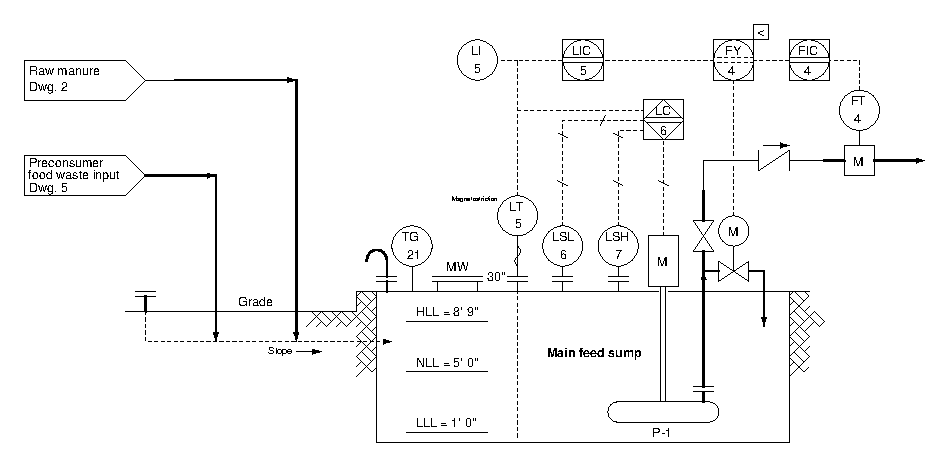
\includegraphics[width=15.5cm]{i00921x05.eps}$$ 













\vfil \eject

\noindent
{\bf Lab questions}

\vskip 20pt

\item{} Sketch connecting wires to make this a working control system.  You should only sketch {\it wires}, as no additional components are necessary:

$$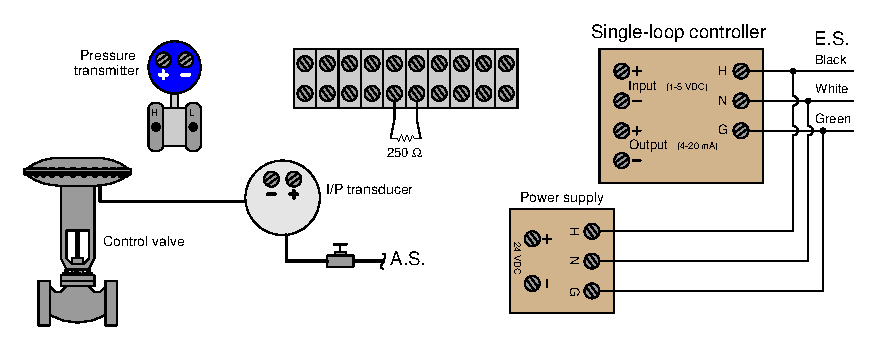
\includegraphics[width=15.5cm]{i00921x07.eps}$$ 

\vskip 20pt

\item{} Identify a practical application for {\it feedforward} control and explain how it works.

\vskip 20pt

\item{} Calculate the pneumatic pressure in a 3-15 PSI range corresponding to 45 percent.

\vskip 20pt

\item{} There is a problem in the control system shown below for the feed sump on an anaerobic digester, which produces methane gas fuel from farm manure and food waste.  The operator reports a low liquid level shown by indicator LI-5 (reading 0 feet 7 inches), and the pump (P-1) not running.  A technician you are working with proposes you take a manual level measurement in the tank using a ``dipstick'' inserted into the sump through a vent pipe to verify the indication shown by LI-5.  Explain what this diagnostic test would tell us about the nature and location of the fault if (1) it did provide a low-level reading in agreement with LI-5, and (2) if it instead showed a normal or high-level reading in disagreement with LI-5.  Be sufficiently detailed in your answer that someone would have a general idea of where the fault was located based on each of your conclusions:

$$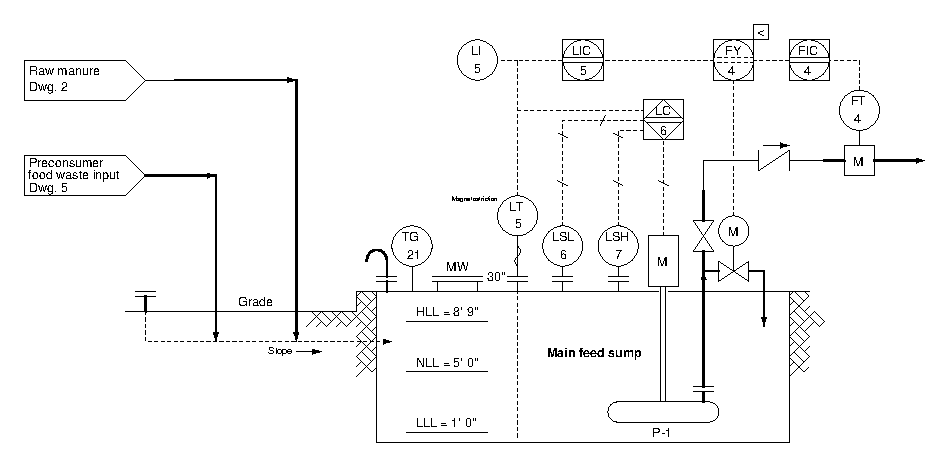
\includegraphics[width=15.5cm]{i00921x05.eps}$$ 

%INDEX% Lab exercise, cascade/ratio/feedforward control strategy

%(END_NOTES)


